%!TEX root = ../dissertation.tex
\begin{savequote}[75mm]
HAMLET: Do you see yonder cloud that’s almost in shape of a camel?\\
POLONIUS: By th' mass, and ’tis like a camel indeed.\\
HAMLET: Methinks it is like a weasel.\\
POLONIUS: It is backed like a weasel.\\
HAMLET: Or like a whale.\\
POLONIUS: Very like a whale.\\
\qauthor{Shakespeare -- Hamlet, Act 3, Scene 2}
\end{savequote}


\chapter{Dynamics of structure and content across repeated reference}
\graphicspath{{./figures/tangrams/}}

\newthought{Lorem ipsum dolor sit amet}, Communication poses a challenging coordination problem for social agents. 
While a lifetime of learning the conventions of our language community provides a crucial backbone for understanding each other \cite{Lewis69_Convention}, we frequently find ourselves in situations where our existing lexicon falls short.
For one, no two speakers share exactly the same lexicon \cite{Davidson86_DerangementOfEpitaphs, Clark98_CommunalLexicons}. 
Lingo, proper nouns, nicknames, slang, inside jokes, metaphors, and other creative uses of neologism all operate in a regime of uncertainty where the same word or phrase may \emph{a priori} mean something different (or nothing at all) to different partners in different contexts. (cite, cite).
At the same time, because we live in a changing environment, we constantly experience novel entities, events, thoughts, and feelings we want to talk about---complex referents for which we have no pre-existing conventions and real uncertainty about whether a novel compositional expression will mean to our partner exactly what we intend it to mean.
What do we do when our lexicon isn't sufficient --- when we have to talk about something we've never had to talk about before with a partner we've never met?

A family of interactive communication experiments called \emph{repeated reference games} have provided a natural and productive paradigm for studying language use in such scenarios. In a seminal study by \cite{KraussWeinheimer64_ReferencePhrases}, pairs of participants played a cooperative language game where they were presented with arrays of ambiguous shapes in randomized orders. 
The players were allowed to talk freely; their goal was to find the correspondence between their boards by producing mutually understood descriptions of the shapes. 
Critically, as particular shapes reappeared on successive rounds of the game, descriptions were dramatically shortened: a lengthy early description like ``the upside-down martini glass in a wire stand'' became simply ``martini'' by the end. 
In other words, these results suggested that speakers addressed the computational challenge of referring to novel objects with a novel partner by initially drawing on many sources of prior information from existing conventions and then \emph{adapting} with their partner based on shared history.

This signature reduction effect has been replicated under many conditions testing the boundaries of adaptation, manipulating the kinds of objects used as targets, the contexts in which the objects appear, the identity of one's partner across repetitions, the feedback available, and the medium participants use to communicate. (cite, cite, cite). 
While this canon of qualitative effects has played an influential role in shaping theories of social coordination in communication, particularly in debates over the role of common ground representations, a \emph{quantitative} characterization of precisely what gets reduced, and how, has remained elusive. 
Yet these details matter for a number of open questions. 
How systematic is the structure of changes over time?
To what extent are idiosyncratic\dots
\todo[inline]{Refine these questions}

Here we present a large corpus of utterances from a web-based 

\todo[inline]{Motivate focus on structure and content; set up alternative hypotheses}

\emph{Arbitrariness} is a definitional property of conventions (Lewis,
1969): there must be multiple solutions that would be equally successful
as long as both players ``agree'' (e.g.~driving on the left vs.~right
side of the road). By the final round in a language game, for example,
the same tangram might be called the `dancer' to one pair and the
`skater' to another. The other definitional property we consider is
\emph{stability}: it is in everyone's best interest to keep using the
convention, once established. Finally, \emph{reduction} is more specific
to the reference game paradigm and refers to the transformation of
longer, complex expressions into simpler expressions over the course of
interaction, as Krauss \& Weinheimer (1964) observed. While this broad
phenomenon has been replicated many times, exactly what is reduced
remains an open empirical question.

Theories of convention-formation differ primarily in the extent to which
sophisticated social reasoning and common ground is required. At one
extreme, agents use simple heuristic updating rules and do not need to
represent or reason about other agents at all (Barr, 2004; Centola \&
Baronchelli, 2015; Young, 2015). Simulations elegantly show how
arbitrary signaling systems can spread and come to dominate large
populations. However, due to their `rich get richer' dynamic, it is not
clear how emergence-through-use mechanisms alone could account for
reduction in repeated interaction. At the other extreme, are theories in
which agents explicitly consider their partner's beliefs and track what
information is \emph{mutual knowledge}, often formalized in a game
theoretic setting (Lewis, 1969). Wilkes-Gibbs \& Clark (1992) and others
have proposed that agents engage in a collaborative process of
establishing mutual knowledge, though the mechanisms allowing
conventions to emerge under such conditions have not been instantiated
in a formal model to our knowledge.

%In this paper, we argue for a theoretical position on the spectrum
%between these poles: \emph{conventions form when agents assume
%conventions already exist}. In other words, agents believe there is a
%true lexicon used by other agents but are initially unsure of its
%identity. Through their interactions with a partner who is assumed to be
%knowledgeable and informative, agents can learn this true lexicon even
%though their partner in fact begins in the same state of ignorance.
%Agents thus coordinate on the same lexicon, which becomes conventional.

%To support this theory, we first conducted a large-scale, multi-player
%replication of the tangrams task, which has traditionally been limited
%to relatively small sample sizes in the lab. We then demonstrate signatures
%of arbitrariness, stability, and reduction which have been difficult to
%study at a fine-grained level due to the sparseness of existing data.
%Next, we formulate our theory in a computational model of communication
%in repeated reference games, based on recent successes capturing
%language understanding as social inference (Goodman \& Frank, 2016;
%Goodman \& Stuhlmüller, 2013) and show that this model qualitatively
%produces all three empirical signatures.

\section{Methods}

\begin{figure}
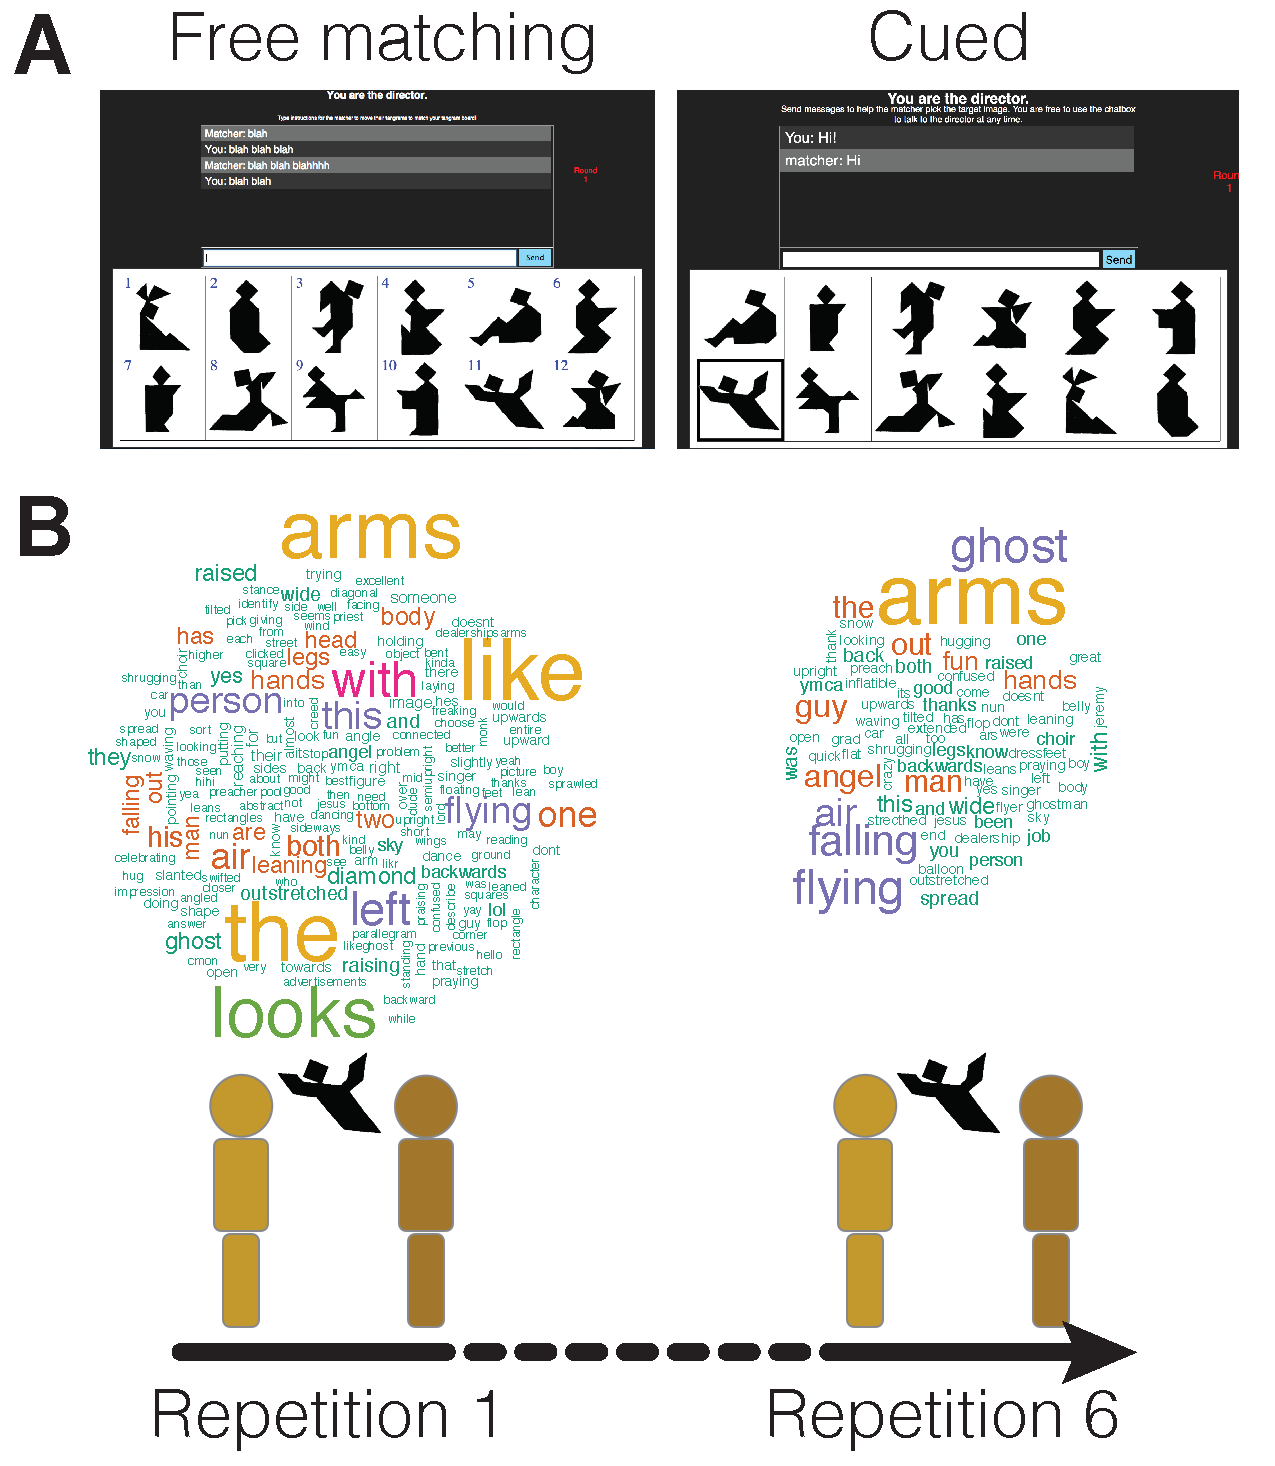
\includegraphics[scale=.65]{designAndExample.pdf}
\caption[Experimental design and example messages]{(A) Screenshots of the `free matching' and `cued' variants of the tangrams task; (B) Visualization of words used to refer to one tangram on the first round compared to the final round. \todo[inline]{Fix text/formatting in screenshots (maybe use scheme instead); think about less corny representation than wordcloud? figure out where to put the wavy guy, maybe add speech bubble to indicate words came from speaker?}}
\label{fig:design}
\end{figure}
\afterpage{\clearpage}

\subsection{Data collection}

To collect a large corpus of natural dialogue that supports quantitative analyses of convention formation over time, we implemented the classic tangrams task used in \cite{ClarkWilkesGibbs86_ReferringCollaborative} in a real-time, multi-player web environment. 
We developed two variants of the game: a \emph{free-matching} version that closely replicates classic in-lab designs and a more tightly controlled \emph{cued} version that allows for higher resolution analyses of how references to individual tangrams changed over time (see Fig. \ref{fig:design}). 
The \emph{free-matching} version was an exploratory sample, but we pre-registered our full pre-processing and analysis pipeline for the \emph{cued} version\footnote{osf.io/XXXXX}, so while we report results for both versions throughout, we privilege the \emph{cued} version as our confirmatory sample.

\subsubsection{Participants}\label{participants}

A total of XXX participants (YYY in the \emph{free-matching} version and ZZZ in the \emph{cued} version) were recruited from Amazon's Mechanical Turk and paired into dyads to play a real-time communication game using the framework in \cite{Hawkins15_RealTimeWebExperiments}. 
We excluded games that terminated before the completion of the experiment, and where participants reported a native language different from English, leaving a corpus of X complete games with a total of X utterances.

\subsubsection{Stimuli \& Procedure}\label{stimuli}

Throughout the task, participants were shown a \(6 \times 2\) grid containing twelve tangram shapes, reproduced from \cite{ClarkWilkesGibbs86_ReferringCollaborative}.  
After passing a short quiz about task instructions, participants were randomly assigned the role of either `director' or `matcher' and automatically paired into virtual rooms containing a chat box and grid of stimuli. 
Both participants could freely use the chat box to communicate at any time. 

In the \emph{free-matching} version, our procedure closely followed \cite{ClarkWilkesGibbs86_ReferringCollaborative}. 
The director and matcher began each round with scrambled boards. 
The director's tangrams were fixed in place, but the matcher's could be clicked and dragged into new positions.
The players was instructed to communicate through the chat box such that the matcher could  rearrange their shapes to match the order of the director's board.
When the players were satisfied that their boards matched, the matcher clicked a `submit' button that gave players batched feedback on their score (out of 12) and scrambled the tangrams for the next round. 
After six rounds, players were redirected to a short exit survey. 
Cells were labeled with fixed numbers from one to twelve in order to help participants easily refer to locations in the grid (see Fig. \ref{fig:design}).

While this replicated design allows for highly naturalistic interaction, it poses several problems for text-based analyses. First, utterances must contain not only descriptions of the tangrams but also information about the intended location (e.g. '\emph{number 10} is the \dots'). Additionally, because there are no constraints on the sequence, participants can revisit tangrams out of order or mention multiple tangrams in a single message, making it difficult to isolate exactly which utterances referred to which tangrams without extensive hand-annotation. Finally, the design of the `submit' button makes it easy for players to occasionally advance to the next round without referring to all 12 tangrams. 

For the \emph{cued} version, then, we designed a straightforwardly sequential variation on the task where speakers are privately cued to refer to targets one-by-one and feedback is given on each round; this allows us to straightforwardly conduct analyses at the tangram-by-tangram level. On each trial, one of the twelve tangrams was privately highlighted for the director with a box as the \emph{target} (see Fig. \ref{fig:design}A). Instead of clicking and dragging into place, matchers simply clicked the one they believed was the target. They were not allowed to click until after a message is sent by the speaker.  We constructed a sequence of six blocks of twelve trials (for a total of 72 trials), where each tangram appeared once per block.%, and the same tangram was never the target twice in a row. 
Because targets were cued one at a time, numbers labeling each square in the grid were irrelevant and we removed them. The context of tangrams was scrambled on every trial, and participants were given full, immediate feedback: the director saw which tangram their partner clicked, and the matcher saw the intended tangram.

\subsection{Data pre-processing}

We used a three step pre-processing pipeline to prepare our corpus for subsequent analyses. Unless otherwise noted, we used the open-source Python package \texttt{spaCy} to implement all NLP tasks. 

\begin{enumerate}

\item \textbf{Spell-checking and regularization}: We conservatively extracted all tokens that did not exist in the vocabulary of the smallest available ($\sim$ 50,000 word) \texttt{spaCy} model and passed them through the SymSpell spell-checker \footnote{\texttt{https://github.com/wolfgarbe/SymSpell}}. These suggested corrections were then sequentially presented to the first author and either accepted or overridden at their judgement. This process constructed a reproducible spell-correction dictionary we applied to our dataset.

\item \textbf{Cleaning unrelated discourse}: Because we allowed our participants to interact in real-time through the chat box, many pairs produced text unrelated to the task of referring to the current target (e.g. greeting one another, asking personal questions, commenting on the length of the task or the results of previous rounds). We wanted to ensure that our structural results were not confounded by patterns in this kind of discourse across the task, and that the semantic content we observe on a particular trial is in fact being used to refer to the current target rather than task-irrelevant topics or, as we found in some cases, referring to other tangrams while debriefing previous errors. We therefore applied a manual pass applying a rubric that any text not directly referring to the current target is removed. For example, utterances like ``this is the one we got wrong last time'' were kept in because they were referring to a property of the current tangram, but utterances like ``good job'' and ``they'll go quicker if you remember what I say!'' are not. This process also created a reproducible JSON.

\item \textbf{Collapsing multiple messages within a round}: Finally, some speakers used our chat box like an texting interface, hitting the enter key between every micro-phrase of text. This made it difficult to interpret the output of syntactic parses. We therefore collapsed repeated messages by a participant within a round into a single message by inserting commas between successive messages. We chose to use commas because it tends to maintain grammaticality and does not inflate word counts.

\end{enumerate}

\subsection{Exclusion criteria}

Because the classic work using the repeated reference game paradigm reported near ceiling accuracy for all pairs, and because the phenomenon we focus on here is not \emph{whether} people can communicate but \emph{how} they do it conditioned on being successful, we pre-registered an exclusion criterion based on accuracy. 
Specifically, we implemented a 66/66 rule, excluding pairs that got got fewer than 66\% tangrams correct (8 of 12) on fewer than 66\% of blocks (4 of 6). 
While the majority of pairs (X\%) were at ceiling accuracy by the final round, this excluded K pairs who on examination of their text appeared to be guessing or rushing to completion.

Still, we verified that all results reported were robust to these exclusion criteria, and to our data pre-processing steps\todo{check}.

\section{Quantifying the dynamics of structure}\label{results}

\subsection{Reduction in dialogue}\label{listener-feedback}

Before narrowing our analysis to the rich properties of \emph{director} referring expressions over time, we first examine the broader dynamics of director-matcher dialogue exchanges. 
An influential result from \cite[see also \cite{KraussWeinheimer66_Tangrams, GarrodFayLeeOberlanderMacLeod07_GraphicalSymbolSystems}]{ClarkWilkesGibbs86_ReferringCollaborative} is that ad hoc conventions for referring are established \emph{collaboratively}: 
directors and matchers engage in a bi-directional process where matchers ask follow-up questions, suggest corrections, and acknowledge or verbally confirm their understanding through a backchannel. 
This theory predicts that (1) listener feedback should be highest on the first round and drop off once meanings are agreed upon, and (2) dyads with more initial listener feedback should reduce to more efficient conventions. 
Our use of a chat box rather than in-person verbal communication, along with the automatic feedback we provided each round in the \emph{cued} condition, may have diminished the bi-directionality somewhat, but we find correlational evidence of both patterns in our uncollapsed but otherwise cleaned data. 
The number of listener messages decreases significantly over the game $(b=-0.5, t = -10.6, p < 0.001)$, and there is a small but significant effect of the (logged) number of initial listener messages on overall \% reduction in the number of words used by the director, $r = 0.26, 95\% CI = [0.57, 0.45], p = 0.014$.
\todo[inline]{Note: this last result isn't actually saying much because when listeners say more on the first round, speaker often say more in response\dots they therefore have a higher initial word count to reduce from than if the listener didn't say anything, so it's not surprising that \% reduction is larger... we need to revise the analysis to control for this, e.g. by only considering reduction from the words used \emph{before} the listener's first message, i.e. what they \emph{would} have initially said if the listener didn't chime in? The more simple \& obvious regression formulation would be whether \# of initial listener messages predicts \emph{absolute} round 6 message length rather than \% reduction; this didn't come out, but I switched to the \% reduction version because I was worried that it was just due to pair-level variance in final round length}
\todo[inline]{This could also be a good place to put an effect of, like, more words used for tangrams that were incorrect in the previous round.}

\begin{figure}[t]
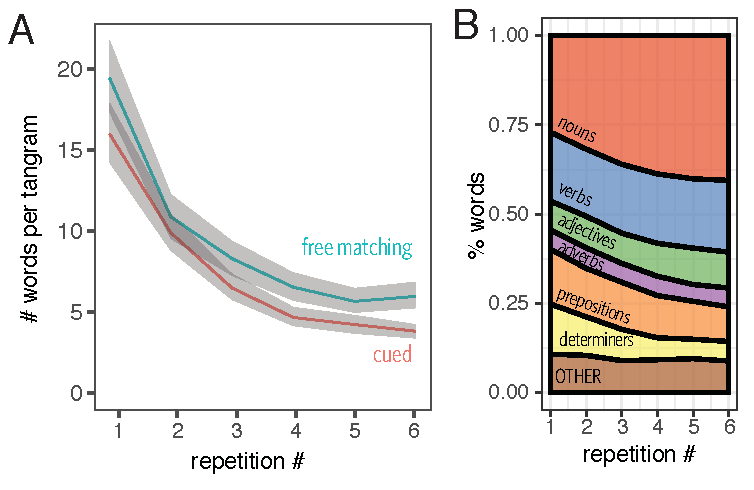
\includegraphics[scale=.65]{reduction.pdf}
\caption{(A) similar reduction in \# words per tangram for both variants of the task (B) word counts broken down by part of speech, combined across both variants (C) phrasal reduction based on syntactic parse \todo[inline]{Maybe showing \% reduction is better than raw numbers, i.e. normalizing by occurrence on first round (or version mike suggested w/ bars showing proportions at beginning and end.}}
\label{fig:reduction}
\end{figure}

\subsection{Reduction in number of words}\label{reduction}

Next, we turn to a set of analyses examining reduction in utterance
length over the course of the experiment. At the coarsest level, we find
that the mean number of words used by speakers decreases over time (see
Fig. \ref{fig:replication}). This decrease replicates a highly reliable
reduction effect found throughout the literature on iterated reference
games (Brennan \& Clark, 1996; Krauss \& Weinheimer, 1964), although
perhaps due to our purely textual (vs.~spoken) interface, participants
in our task used many fewer words overall than previously reported. The
following analyses break down this broad reduction into a finer-grained
set of phenomena.

\subsection{Reduction in parts of speech}
The next level of granularity motivating our model approach concerns
which kinds of words are most likely to be dropped. Is the speaker
adopting a shorthand where they drop uninformative function words, or
are they simplifying or narrowing their descriptions by omitting
meaningful details (Clark \& Wilkes-Gibbs, 1986)? We used the Stanford
CoreNLP part-of-speech tagger (Toutanova, Klein, Manning, \& Singer,
2003) to count the number of words belonging to each part of speech in
each message. Fig. \ref{fig:pos} shows the percent reduction of
different parts of speech from the first round to the sixth round. We
find that determiners (`the', `a', `an') are the most likely class of
words to be dropped with an X\% reduction rate, on average. Nouns
(`dancer', `rabbit') are the least likely class to be dropped with only
an Y\% rate. Closed-class parts of speech are strictly more likely to be
dropped than open-class parts of speech.

While this finding suggests that speakers might just be adopting a
shorthand using more ungrammatical fragments as the game proceeds, we
find a more complex dynamic by examining the table of unigrams and
bigrams most likely to be dropped (see Table \ref{tab:words}). Note that
alongside dropped articles, there are a number of words that form
conjunctions (`and') and modifiers (`of', `with', `the right'). In other
words, it may be more likely that when function words are dropped, it is
primarily as part of larger grammatical units that provide additional
information in identifying the target.

\subsection{Reduction in syntactic constituents}
We explicitly examined this hypothesis by running the Stanford
constituency parser (Schuster \& Manning, 2016), tagging the occurrence
of subordinate/adverbial clauses (`sitting \emph{facing left}') and
adjectival clauses (`angel \emph{that is praying}').\footnote{Specifically,
  we used the Universal Dependencies tags \texttt{csubj, ccomp, xcomp},
  and \texttt{advcl} for subordinate clauses and \texttt{acl} for
  adjectival clauses (Schuster \& Manning, 2016)} We found that both
were reduced over the course of the game (see Fig.
\ref{fig:replication}), lending additional support for the hypothesis
that meaningful details are increasingly omitted. Initial phrases pile
on multiple ambiguous, partially redundant modifiers and descriptors: as
the game progresses and ambiguity of reference decreases, these
additional meaningful units become less useful and can be dropped.

This result accords with early observations by \cite{Carroll80_NamingHedges}, which found that in three-quarters of transcripts from \cite{KraussWeinheimer64_ReferencePhrases} the short names that participants converged upon were prominent in some syntactic construction at the beginning, often as a head noun that was initially modified or qualified by other information. 

\subsection{Shared dynamics across pairs}

Tree-edit distance\dots

\begin{figure}[t]
\centering
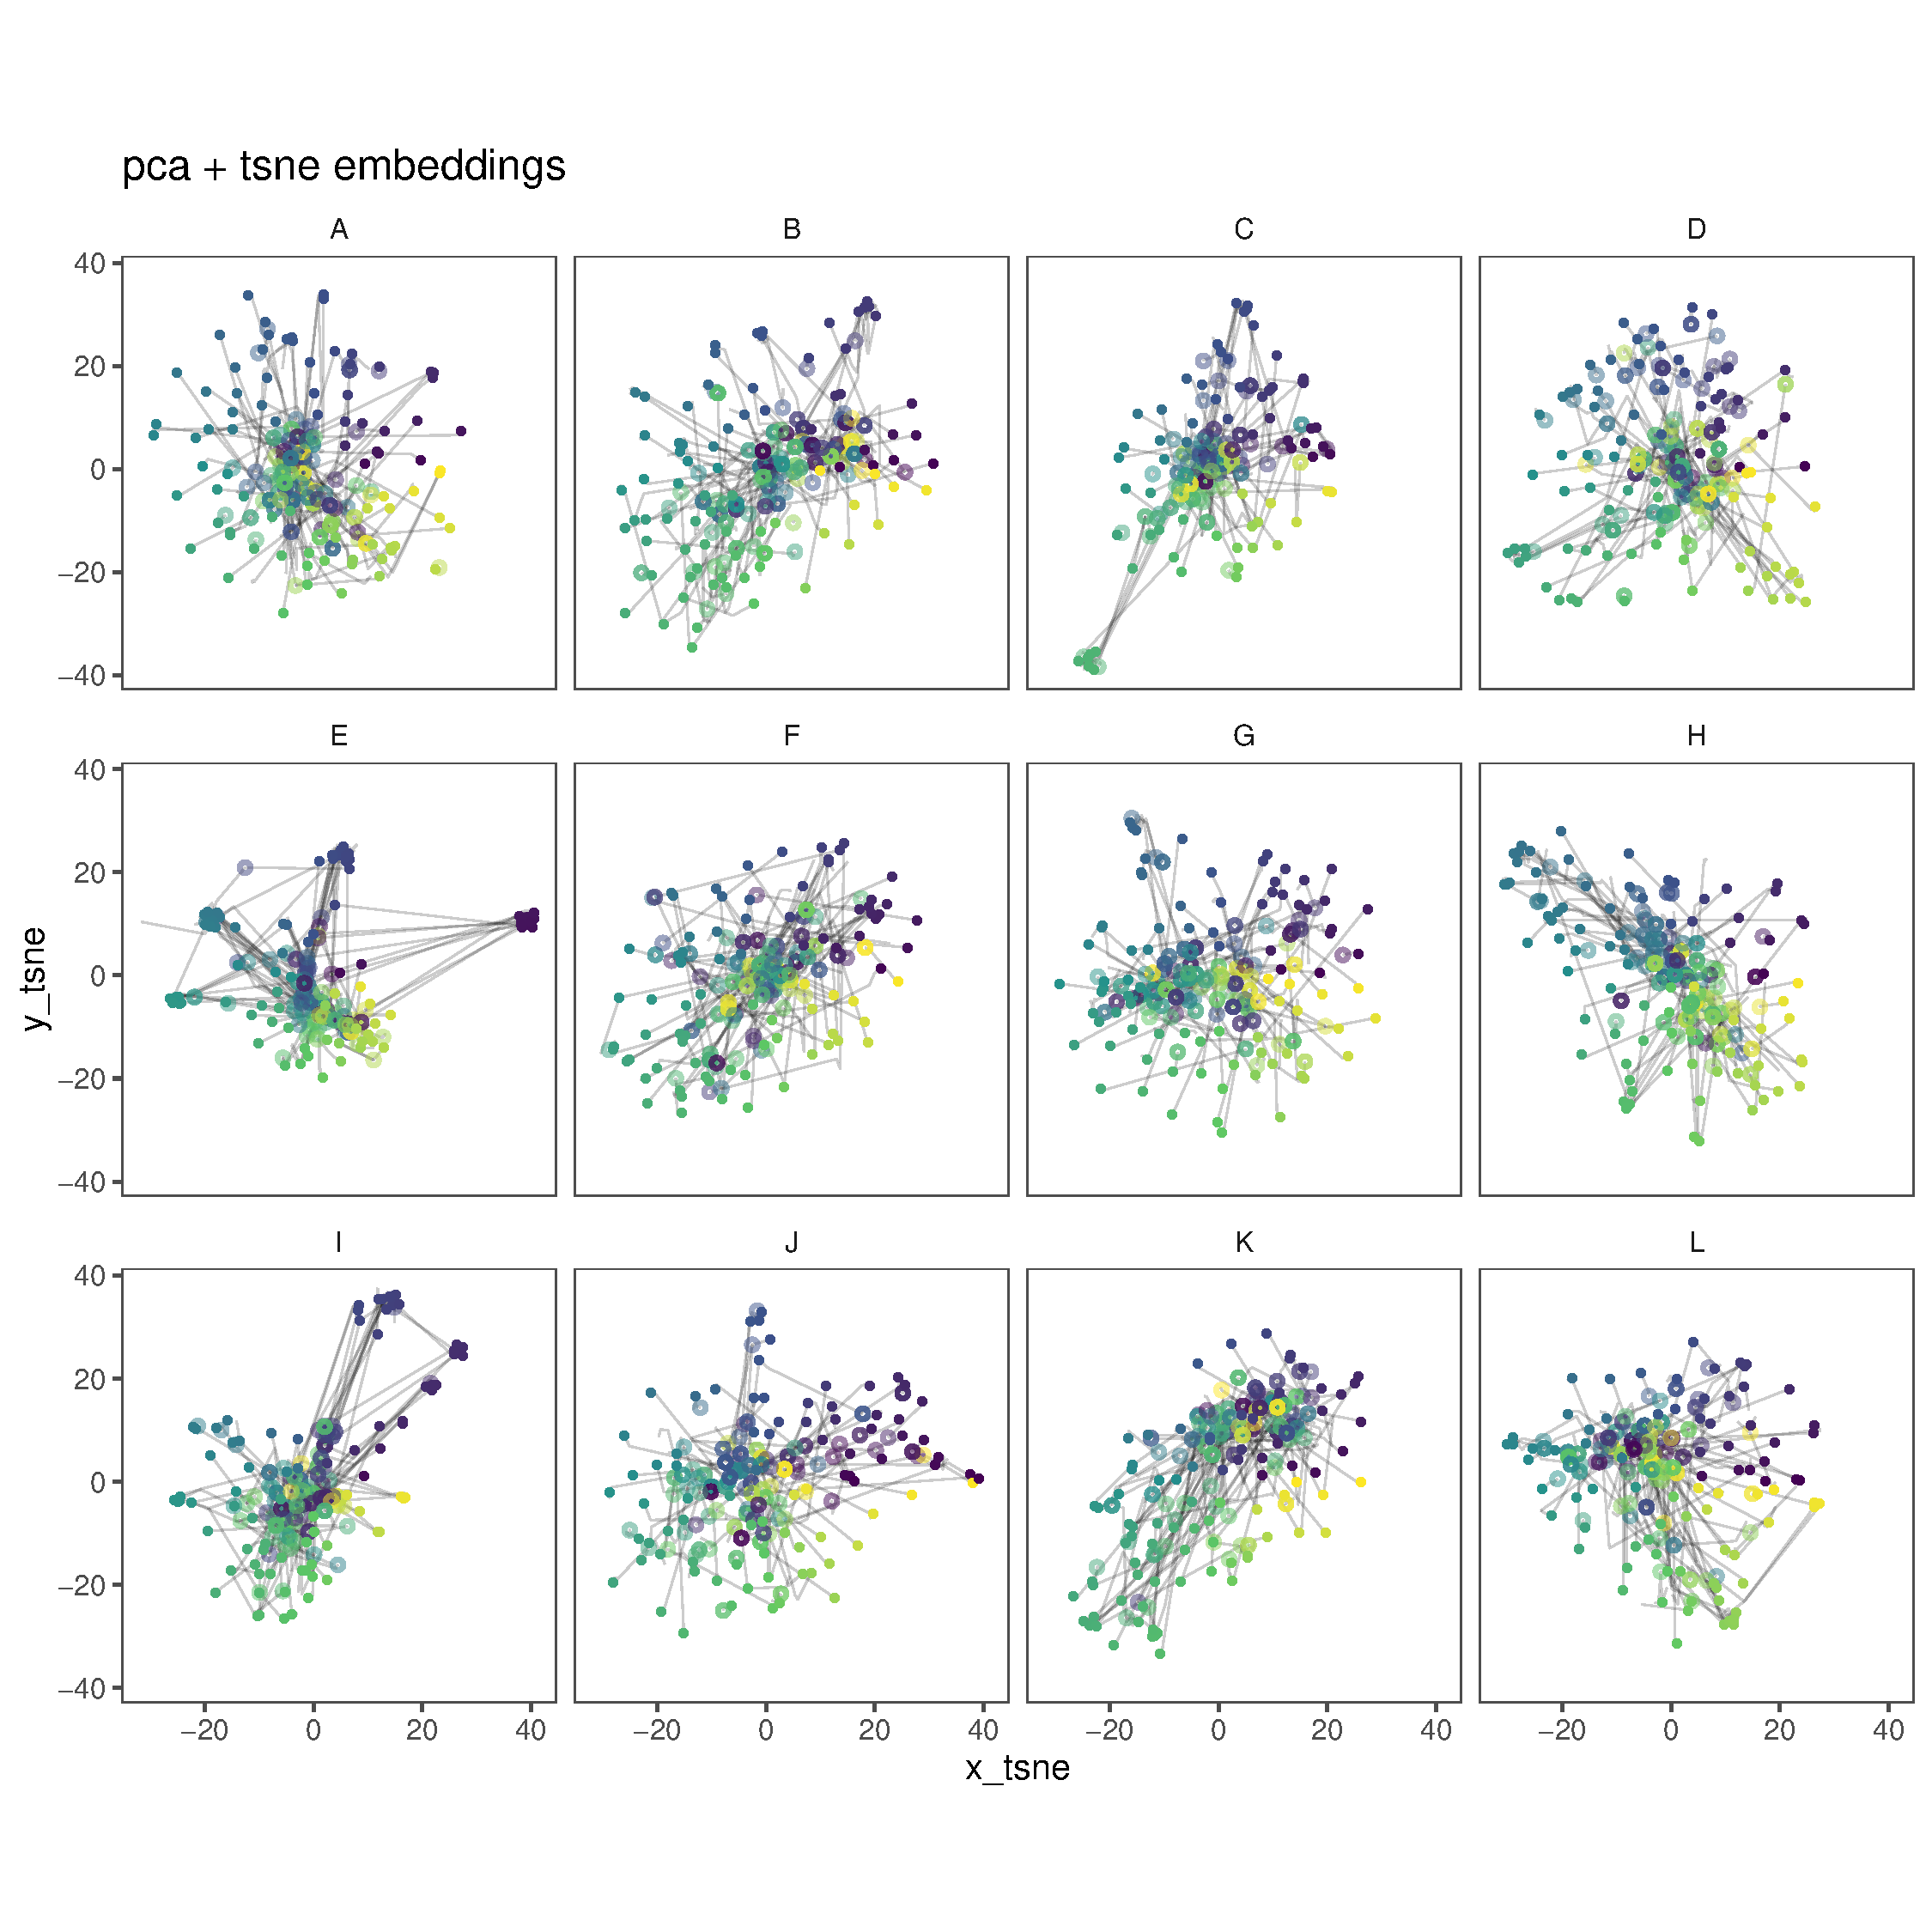
\includegraphics[scale=.3]{tsne_embeddings.pdf}
\caption{Semantic embeddings of referring expressions for each tangram, as they change over the game. \todo[inline]{Without really zooming in, it's harder to see the open/closed circles indicating beginning/end (color dominates)}}
\label{fig:reduction}
\end{figure}

\section{Quantifying the dynamics of content}

\subsection{Idiosyncracy across pairs, stability within pairs}
\label{arbitrariness-and-stability}

We begin by examining signatures of \emph{arbitrariness} and
\emph{stability} in our data. We operationalize these concepts using the
information-theoretic measure of entropy:
\[H(W) = \sum_w P(w) \log P(w)\] Broadly speaking, entropy measures the
predictability of a distribution. It is maximized when all elements are
equally likely and declines as the distribution becomes more structured,
i.e.~when the probability mass is concentrated on a subset of elements.

To derive predictions, we consider a permutation-test null model in
which utterances are scrambled within each round. The empirical entropy
of individual games should only differ from the null distribution if
\emph{both} arbitrariness and stability hold. First, note that if
stability did \emph{not} hold, scrambling would have no effect on the
entropy within individual games: speakers would already use different
words each round, and swapping out the identity of those words would not
affect the entropy of the word distribution.

If stability holds but arbitrariness does not, all players would adopt
the single optimal (non-arbitrary) way to refer to each tangram.
Therefore, the entropy of their word distributions also should not be
affected by scrambling: a speaker's real words would be swapped out for
the same words, just generated by another speaker. Finally, if both
arbitrariness and stability hold, then different speakers adopt
different referring expressions that persist from round to round. Hence,
scrambling should \emph{increase} the average game's entropy from a
relatively low level: each game's idiosyncratic, concentrated
distribution of words would be mixed together to form more heterogeneous
and therefore high-entropy distributions.

To test this prediction, we computed the average within-game entropy for
1000 different permutations of speaker utterances. We permuted
utterances within rounds rather than across the entire data set to
control for the fact that earlier rounds have longer utterances and thus
a larger vocabulary than later rounds (see the following section). Since
this permutation scheme keeps the number of messages per participant
constant and simply swaps out the content of those messages, it also
controls for the fact that some speakers sent more messages than others.
We found that our null distribution lay within the interval {[}X, Y{]},
which is significantly higher than the true entropy (averaged across
games) of Z \(p < 0.001\). This pattern is consistent only with
signatures of both arbitrariness and stability.

\subsection{Point-wise Mutual Information}

Which words are dropped and which remain?

\subsection{Semantic embeddings}\label{arbitrariness-and-stability}

While words can be treated as discrete tokens, as in the previous section, \dots

Idiosyncracy across pairs can additionally be assessed by testing the generalization performance of a classifier on held out pairs at the beginning and end of the game. Training on earlier \dots

\section{General Discussion}\label{general-discussion}

In this paper, we revisited the classic phenomenon of
convention-formation in a large-scale replication of the tangrams task,
finding evidence of arbitrariness and stability as well as finer-grained
reduction of meaningful clauses. 

%% Paragraph about opportunities for computational models
While we have focused on broader theoretical questions, our results also serve as a foundation for high-resolution task-performing computational models of communication seeking to explain the full richness of natural data. To build machines that naturally adapt to their interlocutors in human-robot or human-computer interaction scenarios, we must go behind qualitative efforts.

Theories of convention-formation vary in the extent to which social
reasoning about common ground is required. Our agents lie on a spectrum
between the heuristic updating agents of Barr (2004) and the
sophisticated agents of Clark \& Wilkes-Gibbs (1986), who
collaboratively build up explicit representations of mutual knowledge.
Speakers and listeners in our model implicitly coordinate their beliefs
through a shared history of observations, which serves as ``common
ground'' in an informal sense. They make critical use of pragmatic,
social reasoning in order to learn meanings, but do not explicitly
consider the fact that this history is shared, or represent their
partner's own uncertainty.

By capturing reduction, which purely heuristic theories have not yet
demonstrated, we showed that minimal assumptions of social reasoning go
a long way in accounting for key phenomena. Still, our model falls short
in some ways. For instance, because we do not provide a mechanisms for
the listener agent to respond with confirmation, repair, or follow-up
questions, we cannot make explicit predictions about the reduction in
\emph{listener messages} (as in Fig. \ref{fig:replication}) or the
impact of early listener responses on conventionalization. These
phenomena require our model to deal with planning over extended
dialogues, and to potentially weaken the assumption that one's partner
knows the true lexicon with complete certainty. Similarly, while our
model was explicitly designed with linguistic conventions in mind, it
remains to be seen whether the same formulation generalizes to broader
behavioral conventions. For example, the real-time coordination games
used in Hawkins \& Goldstone (2016) may not require players to reason
about a structured lexicon with noise, but an action policy
representation may play a similar role. While there remain many complex
aspects of convention-formation in communication games left for future
research, our approach nonetheless serves as a lower bound on the degree
of social reasoning needed to capture lexical conventions in these
games.
